%! Licence = CC BY-NC-SA 4.0

%! Author = mariuszindel
%! Date = 24. Jan 2021
%! Project = latex-test-template


%import template
%! Licence = CC BY-NC-SA 4.0

%! Author = mariuszindel
%! Date = 24. Jan 2021
%! Project = latex-test-template

\documentclass[a4paper, landscape, fontsize=10pt]{scrartcl} %-scrartcl = deutsche Sprache

% charset
\usepackage[T1]{fontenc}
\usepackage[utf8]{inputenc} %-inputenc = Umlaute möglich
\usepackage{ulem}

% use language german
\usepackage[ngerman]{babel} % with n is new spelling

% format page size
\usepackage{geometry}
\geometry{top=0.25cm,left=0.25cm,right=0.25cm,bottom=0.25cm}
%\textheight = 558pt

% tabular
\usepackage{tabularx}

% math
\usepackage{amsmath}
\usepackage{amssymb}
\usepackage{amsfonts}
\usepackage{enumitem}

% graphic
\usepackage{graphicx}
\graphicspath{{media/}}

% colors
\usepackage[dvipsnames]{xcolor}

% multi columns
\usepackage{multicol}

% make items compact
\setlist{topsep=0pt, leftmargin=3mm, nolistsep}
\setlength{\parindent}{0cm} % disable indention of text

% author and institute
\newcommand{\AUTHOR}{Marius Zindel }
\newcommand{\INSTITUTE}{Hochschule für Technik Rapperswil}

% define header and footer
\usepackage{fancyhdr}
\pagestyle{fancy}

%\fancyhead[RO]{\AUTHOR| \INSTITUTE}
%\fancyhead[LO]{\TITLE}
%\fancyfoot[RO]{\DELIVERYDATE}
%\fancyfoot[LO]{Created with \LaTeX}
\renewcommand\headrulewidth{0pt}
\renewcommand\footrulewidth{0pt}
%\headsep = -2pt
\footskip = 0pt

% define color
\definecolor{sectionColor}{HTML}{228B22}
\definecolor{subSectionColor}{HTML}{CB4154}
\definecolor{subSubSectionColor}{HTML}{FFFF00}
\definecolor{inlineCodeColor}{HTML}{FF00FF}
\definecolor{codeBackground}{RGB}{245,245,245}
\definecolor{gray}{rgb}{0.5,0.5,0.5}
\definecolor{darkGreen}{RGB}{0,150,0}
\definecolor{DarkPurple}{rgb}{0.4, 0.1, 0.4}

% define section format
\usepackage{sectsty}
\usepackage{titlesec}

\titleformat{name=\section}[block]{\sffamily\small}{}{0pt}{\colorsection}
\titlespacing*{\section}{0pt}{0pt}{0pt}
\newcommand{\colorsection}[1]{%
    \colorbox{sectionColor!40}{\parbox{0.98\linewidth}{\color{black}\thesection\ #1 }}} % 0.235\textwidth

% define subsection format
\titleformat{name=\subsection}[block]{\sffamily\small}{}{0pt}{\colorsubsection}
\titlespacing*{\subsection}{0pt}{0pt}{0pt}
\newcommand{\colorsubsection}[1]{%
    \colorbox{subSectionColor!40}{\parbox{0.98\linewidth}{\color{black}\thesubsection\ #1 }}}

% define subsubsection format
\titleformat{name=\subsubsection}[block]{\sffamily\small}{}{0pt}{\colorsubsubsection}
\titlespacing*{\subsubsection}{0pt}{0pt}{0pt}
\newcommand{\colorsubsubsection}[1]{%
    \colorbox{subSubSectionColor!50}{\parbox{0.98\linewidth}{\color{black}\thesubsubsection\ #1 }}}

% import code listings
\usepackage{listings}
\usepackage{beramono}
%! Licence = CC BY-NC-SA 4.0

%! Author = mariuszindel
%! Date = 22. Feb 2021
%! Project = latex-test-template

\definecolor{editorGray}{rgb}{0.95, 0.95, 0.95}
\definecolor{editorOcher}{rgb}{1, 0.5, 0} % #FF7F00 -> rgb(239, 169, 0)
\definecolor{editorGreen}{rgb}{0, 0.5, 0} % #007C00 -> rgb(0, 124, 0)
\definecolor{orange}{rgb}{1,0.45,0.13}
\definecolor{olive}{rgb}{0.17,0.59,0.20}
\definecolor{brown}{rgb}{0.69,0.31,0.31}
\definecolor{purple}{rgb}{0.38,0.18,0.81}
\definecolor{lightblue}{rgb}{0.1,0.57,0.7}
\definecolor{lightred}{rgb}{1,0.4,0.5}
\definecolor{stringstyle}{RGB}{0, 128, 0}

\lstdefinelanguage{CSS}{
    keywords={color,background-image:,margin,padding,font,weight,display,position,top,left,right,bottom,list,style,border,size,white,space,min,width, transition:, transform:, transition-property, transition-duration, transition-timing-function},
    sensitive=true,
    morecomment=[l]{//},
    morecomment=[s]{/*}{*/},
    morestring=[b]',
    morestring=[b]",
    alsoletter={:},
    alsodigit={-}
}

\lstdefinelanguage{JavaScript}{
    morekeywords={typeof, new, true, false, catch, function, return, null, catch, switch, var, if, in, while, do, else, case, break},
    morecomment=[s]{/*}{*/},
    morecomment=[l]//,
    morestring=[b]",
    morestring=[b]'
}

\lstdefinelanguage{HTML5}{
    language=html,
    sensitive=true,
    alsoletter={<>=-},
    morecomment=[s]{<!-}{-->},
    tag=[s],
    otherkeywords={
        % General
        >,
        % Standard tags
        <!DOCTYPE,
        </html, <html, <head, <title, </title, <style, </style, <link, </head, <meta, />,
        % body
        </body, <body,
        % Divs
        </div, <div, </div>,
        % Paragraphs
        </p, <p, </p>,
        % scripts
        </script, <script,
        % More tags...
        <canvas, /canvas>, <svg, <rect, <animateTransform, </rect>, </svg>, <video, <source, <iframe, </iframe>, </video>, <image, </image>, <header, </header, <article, </article
    },
    ndkeywords={
        % General
        =,
        % HTML attributes
        charset=, src=, id=, width=, height=, style=, type=, rel=, href=,
        % SVG attributes
        fill=, attributeName=, begin=, dur=, from=, to=, poster=, controls=, x=, y=, repeatCount=, xlink:href=,
        % properties
        margin:, padding:, background-image:, border:, top:, left:, position:, width:, height:, margin-top:, margin-bottom:, font-size:, line-height:,
        % CSS3 properties
        transform:, -moz-transform:, -webkit-transform:,
        animation:, -webkit-animation:,
        transition:,  transition-duration:, transition-property:, transition-timing-function:,
    }
}


\lstdefinestyle{Java}{
    language=java,
    backgroundcolor = \color{codeBackground},       %color for the background
    keywordstyle=\color{RoyalBlue}\ttfamily,        % style of keywords in source language
    stringstyle=\color{darkGreen}\ttfamily,         % style of strings in source language
    commentstyle=\color{DarkPurple!60}\ttfamily,    % style of comments in source language
    escapeinside={£}{£},                            % specify characters to escape from source code to LATEX
    showspaces=false,                               % emphasize spaces in code (true/false)
    showstringspaces=false,
    showtabs=false,                                 % emphasize tabulators in code (true/false)
    numbers=none,                                   % position of line numbers (left/right/none)
    numberstyle=\tiny\color{darkgray}\ttfamily,     % style used for line-numbers
    stepnumber=1,                                   % distance of line-numbers from the code
    tabsize=1,                                      % default tabsize
    breaklines=true,                                % automatic line-breaking
    breakatwhitespace=true,                         % sets if automatic breaks should only happen at whitespaces
%frame=single,                                   % showing frame outside code (none/leftline/topline/bottomline/lines/single/shadowbox)
    xleftmargin=0pt,
    xrightmargin=-3pt,
    frameround=tttt,                            % enable round corners
    rulecolor = \color{lightgray},              % Specify the colour of the frame-box
    captionpos = b                              % position of caption (t/b)
}

\lstdefinestyle{CSharp}{
    language=[Sharp]C,
    backgroundcolor = \color{codeBackground},       %color for the background
    keywordstyle=\color{RoyalBlue}\ttfamily,        % style of keywords in source language
    stringstyle=\color{darkGreen}\ttfamily,         % style of strings in source language
    commentstyle=\color{DarkPurple!60}\ttfamily,    % style of comments in source language
    escapeinside={£}{£},                            % specify characters to escape from source code to LATEX
    showspaces=false,                               % emphasize spaces in code (true/false)
    showstringspaces=false,
    showtabs=false,                                 % emphasize tabulators in code (true/false)
    numbers=none,                                   % position of line numbers (left/right/none)
    numberstyle=\tiny\color{darkgray}\ttfamily,     % style used for line-numbers
    stepnumber=1,                                   % distance of line-numbers from the code
    tabsize=1,                                      % default tabsize
    breaklines=true,                                % automatic line-breaking
    breakatwhitespace=true,                         % sets if automatic breaks should only happen at whitespaces
%frame=single,                                   % showing frame outside code (none/leftline/topline/bottomline/lines/single/shadowbox)
    xleftmargin=0pt,
    xrightmargin=-3pt,
    frameround=tttt,                            % enable round corners
    rulecolor = \color{lightgray},              % Specify the colour of the frame-box
    captionpos = b                              % position of caption (t/b)
}

\lstdefinestyle{JavaScript}{
    keywords={typeof, new, true, false, catch, function, return, null, catch, switch, var, if, in, while, do, else, case, break},
    ndkeywords={class, export, boolean, throw, implements, import, this},
    comment=[l]{//},
    backgroundcolor = \color{codeBackground},       %color for the background
    keywordstyle=\color{RoyalBlue}\ttfamily,        % style of keywords in source language
    stringstyle=\color{darkGreen}\ttfamily,         % style of strings in source language
    commentstyle=\color{DarkPurple!60}\ttfamily,    % style of comments in source language
    escapeinside={£}{£},                            % specify characters to escape from source code to LATEX
    showspaces=false,                               % emphasize spaces in code (true/false)
    showstringspaces=false,
    showtabs=false,                                 % emphasize tabulators in code (true/false)
    numbers=none,                                   % position of line numbers (left/right/none)
    numberstyle=\tiny\color{darkgray}\ttfamily,     % style used for line-numbers
    stepnumber=1,                                   % distance of line-numbers from the code
    tabsize=1,                                      % default tabsize
    breaklines=true,                                % automatic line-breaking
    breakatwhitespace=true,                         % sets if automatic breaks should only happen at whitespaces
%frame=single,                                   % showing frame outside code (none/leftline/topline/bottomline/lines/single/shadowbox)
    xleftmargin=0pt,
    xrightmargin=-3pt,
    frameround=tttt,                            % enable round corners
    rulecolor = \color{lightgray},              % Specify the colour of the frame-box
    captionpos = b                              % position of caption (t/b)
}

\lstdefinestyle{HTML}{
    language=HTML,
    backgroundcolor = \color{codeBackground},       %color for the background
    keywordstyle=\color{RoyalBlue}\ttfamily,        % style of keywords in source language
    stringstyle=\color{darkGreen}\ttfamily,         % style of strings in source language
    commentstyle=\color{DarkPurple!60}\ttfamily,    % style of comments in source language
    escapeinside={£}{£},                            % specify characters to escape from source code to LATEX
    showspaces=false,                               % emphasize spaces in code (true/false)
    showstringspaces=false,
    showtabs=false,                                 % emphasize tabulators in code (true/false)
    numbers=none,                                   % position of line numbers (left/right/none)
    numberstyle=\tiny\color{darkgray}\ttfamily,     % style used for line-numbers
    stepnumber=1,                                   % distance of line-numbers from the code
    tabsize=1,                                      % default tabsize
    breaklines=true,                                % automatic line-breaking
    breakatwhitespace=true,                         % sets if automatic breaks should only happen at whitespaces
%frame=single,                                   % showing frame outside code (none/leftline/topline/bottomline/lines/single/shadowbox)
    xleftmargin=0pt,
    xrightmargin=-3pt,
    frameround=tttt,                            % enable round corners
    rulecolor = \color{lightgray},              % Specify the colour of the frame-box
    captionpos = b                              % position of caption (t/b)
}

\lstdefinestyle{Python}{
    language=Python,
    backgroundcolor = \color{codeBackground},       %color for the background
    keywordstyle=\color{RoyalBlue}\ttfamily,        % style of keywords in source language
    stringstyle=\color{darkGreen}\ttfamily,         % style of strings in source language
    commentstyle=\color{DarkPurple!60}\ttfamily,    % style of comments in source language
    escapeinside={£}{£},                            % specify characters to escape from source code to LATEX
    showspaces=false,                               % emphasize spaces in code (true/false)
    showstringspaces=false,
    showtabs=false,                                 % emphasize tabulators in code (true/false)
    numbers=none,                                   % position of line numbers (left/right/none)
    numberstyle=\tiny\color{darkgray}\ttfamily,     % style used for line-numbers
    stepnumber=1,                                   % distance of line-numbers from the code
    tabsize=1,                                      % default tabsize
    breaklines=true,                                % automatic line-breaking
    breakatwhitespace=true,                         % sets if automatic breaks should only happen at whitespaces
%frame=single,                                   % showing frame outside code (none/leftline/topline/bottomline/lines/single/shadowbox)
    xleftmargin=0pt,
    xrightmargin=-3pt,
    frameround=tttt,                            % enable round corners
    rulecolor = \color{lightgray},              % Specify the colour of the frame-box
    captionpos = b                              % position of caption (t/b)
}

\lstdefinestyle{bash}{
    language=bash,
    backgroundcolor = \color{codeBackground},       %color for the background
    keywordstyle=\color{RoyalBlue}\ttfamily,        % style of keywords in source language
    stringstyle=\color{darkGreen}\ttfamily,         % style of strings in source language
    commentstyle=\color{DarkPurple!60}\ttfamily,    % style of comments in source language
    escapeinside={£}{£},                            % specify characters to escape from source code to LATEX
    showspaces=false,                               % emphasize spaces in code (true/false)
    showstringspaces=false,
    showtabs=false,                                 % emphasize tabulators in code (true/false)
    numbers=none,                                   % position of line numbers (left/right/none)
    numberstyle=\tiny\color{darkgray}\ttfamily,     % style used for line-numbers
    stepnumber=1,                                   % distance of line-numbers from the code
    tabsize=1,                                      % default tabsize
    breaklines=true,                                % automatic line-breaking
    breakatwhitespace=true,                         % sets if automatic breaks should only happen at whitespaces
%frame=single,                                   % showing frame outside code (none/leftline/topline/bottomline/lines/single/shadowbox)
    xleftmargin=0pt,
    xrightmargin=-3pt,
    frameround=tttt,                            % enable round corners
    rulecolor = \color{lightgray},              % Specify the colour of the frame-box
    captionpos = b                              % position of caption (t/b)
}

\lstdefinestyle{LaTeX}{
    language=TeX,
    backgroundcolor = \color{codeBackground},       %color for the background
    keywordstyle=\color{RoyalBlue}\ttfamily,        % style of keywords in source language
    stringstyle=\color{darkGreen}\ttfamily,         % style of strings in source language
    commentstyle=\color{DarkPurple!60}\ttfamily,    % style of comments in source language
    escapeinside={£}{£},                            % specify characters to escape from source code to LATEX
    showspaces=false,                               % emphasize spaces in code (true/false)
    showstringspaces=false,
    showtabs=false,                                 % emphasize tabulators in code (true/false)
    numbers=none,                                   % position of line numbers (left/right/none)
    numberstyle=\tiny\color{darkgray}\ttfamily,     % style used for line-numbers
    stepnumber=1,                                   % distance of line-numbers from the code
    tabsize=1,                                      % default tabsize
    breaklines=true,                                % automatic line-breaking
    breakatwhitespace=true,                         % sets if automatic breaks should only happen at whitespaces
%frame=single,                                   % showing frame outside code (none/leftline/topline/bottomline/lines/single/shadowbox)
    xleftmargin=0pt,
    xrightmargin=-3pt,
    frameround=tttt,                            % enable round corners
    rulecolor = \color{lightgray},              % Specify the colour of the frame-box
    captionpos = b                              % position of caption (t/b)
}



\lstdefinestyle{htmlcssjs} {
    language=HTML5,
    alsolanguage=JavaScript,
    alsodigit={.:;},
% General design
%  backgroundcolor=\color{editorGray},
    frame=none,
% line-numbers
% xleftmargin={0.75cm},
    numbers=none,
% Code design
    identifierstyle=\color{black},
    backgroundcolor = \color{codeBackground},       %color for the background
    keywordstyle=\color{RoyalBlue}\ttfamily,        % style of keywords in source language
    ndkeywordstyle=\color{editorGreen}\bfseries,
    stringstyle=\color{darkGreen}\ttfamily,         % style of strings in source language
    commentstyle=\color{DarkPurple!60}\ttfamily,    % style of comments in source language
% Code
    tabsize=1,
    showtabs=false,
    showspaces=false,
    showstringspaces=false,
    extendedchars=true,
    breaklines=true,
}



\lstset{style=htmlcssjs}
\lstset{aboveskip=0pt, belowskip=0pt}
\lstset{basicstyle={\footnotesize\ttfamily}}
\lstset{
    literate=  % Allow for German characters in lstlistings.
        {Ö}{{\"O}}1
        {Ä}{{\"A}}1
        {Ü}{{\"U}}1
        {ü}{{\"u}}1
        {ä}{{\"a}}1
        {ö}{{\"o}}1
}

% dotted rule
\usepackage{dashrule}
\usepackage{tikz}
\usetikzlibrary{decorations.markings}
\newcommand{\drule}[3][0]{
    \tikz[baseline]{\path[decoration={markings,
    mark=between positions 0 and 1 step 2*#3
    with {\node[fill, circle, minimum width=#3, inner sep=0pt, anchor=south west] {};}},postaction={decorate}]  (0,#1) -- ++(#2,0);}}

% no indentation
\setlength{\parindent}{0cm}

% include lorem ipsum
\usepackage{lipsum}

\setlist[itemize]{noitemsep, topsep=0pt}

%TODO
\newcommand{\code}{\lstinline[keywordstyle=\color{inlineCodeColor}, basicstyle=\color{inlineCodeColor}, directivestyle=\color{inlineCodeColor}, stringstyle=\color{inlineCodeColor}, identifierstyle=\color{inlineCodeColor}]}





\newcommand{\TITLE}{Test Cheat Sheet}
\newcommand{\DELIVERYDATE}{22.02.2021}

\begin{document}
    \setlength{\columnseprule}{0.4pt}
    \footnotesize
    \begin{multicols*}{4}
        \setlength{\columnseprule}{0.4pt}
        %\footnotesize
        %\tiny

        %! Author = Philipp Emmenegger
%! Date = 30/06/2021

\section{Introduction}
\textbf{Artificial Intelligence (AGI)}
\begin{itemize}
    \item broad concept
    \item different interpretations
    \item we do not have a definition of intelligence
    \item a hypothetical computer program that can perform intellectual tasks as well or better than a human
\end{itemize}
\vspace{10pt}
\textcolor{blue}{Examples of application (today)}
\begin{itemize}
    \item Personalization of news feeds
    \item Product searching and recommendation s on eCommerce platforms
    \item Voice-to-text
    \item Predictive maintenance
\end{itemize}
\vspace{10pt}
\textbf{Statistical machine learning}
\begin{itemize}
    \item Algorithms and applications where computer learn from data
\end{itemize}
\vspace{10pt}
\textbf{Turing Test}
\begin{itemize}
    \item Also called imitation game
    \item Tests of a machine's ability to exhibit intelligent behaviour equivalent to, or indistinguishable from that of a human
    \item Has some philosophical problems (Complex problems, humans cant solve / AI must learn to lie)
\end{itemize}
\vspace{10pt}
\textbf{Bias}
\begin{itemize}
    \item Results that are systematically prejudiced due to faulty assumptions
    \item The inability for a machine learning method (like linear regression) to capture the true relationship, eg. Straight Line can't be curved like the true relationship
\end{itemize}
\vspace{10pt}
\textbf{Variance}
\begin{itemize}
    \item The difference in fits between training and testing set (different data sets in general)
    \item \textcolor{blue}{Low variance} Sum of Squares are very similar for different datasets
\end{itemize}
\vspace{10pt}
\textbf{Predictive modeling}

Train model for predictions \\

\textbf{Feature}

e.g. Years of working experience, school grades

The ideal ML algorithm has low bias and can accurately model the true relationship and it has low variability by producing consistent predictions across different datasets. \\

\textbf{Feature Engineering}
\begin{itemize}
    \item The process of identifying useful, additional input from the data
    \item A typical preprocessing step before the actual learning process starts
\end{itemize}
\vspace{10pt}
\textbf{Deep neural network}

ANNs with multiple hidden layers \\

\subsection{Tasks and Algorithms of Machine Learning}
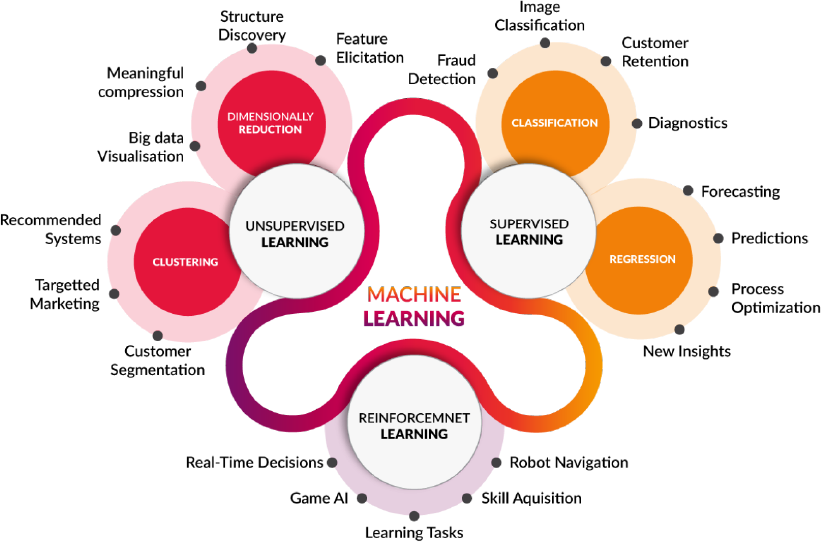
\includegraphics[width=\linewidth]{machine_learning_sections.png}

\subsection{7 Steps of Machine Learning}
\begin{enumerate}
    \item \textcolor{blue}{Gathering data} Collect quantity/quality data for training/testing
    \item \textcolor{blue}{Preparing that data} Cleanup data (remove duplicates, correct errors, deal with missing values, normalize data, convert data types)
    \item \textcolor{blue}{Choosing a model} Select the right algorithm(s)
    \item \textcolor{blue}{Training} Train the model, each iteration of process is a training step
    \item \textcolor{blue}{Evaluation} Use metrics to measure objective performance of the model, test model against previously unseen data, good train/eval split is 80/20, 70/30
    \item \textcolor{blue}{Hyperparameter tuning} Try to improve upon the positive results achieved during the evaluation through gamble with stepNumber of training steps, learning rate, initialization values and distribution
    \item \textcolor{blue}{Prediction} Model should be ready for practical applications
\end{enumerate}

        \columnbreak
        \section{Natural Language Processing (NLP)}
\begin{itemize}
    \item Automated processing of human language (written \& spoken)
    \item Aims to understand and generate human (natural) language
    \item Understanding spoken text is still difficult
    \item Understanding written text became BIG business (search-engines)
    \item Generating human-like conversations is still very hard
\end{itemize}
\subsection{4 Ingredients of Machine Learning}
\textbf{1. Data}
\begin{itemize}
    \item Dataset
    \item Pre-Processing Pipeline including cleansing, feature-engineering, data augmentation etc.
\end{itemize}
\textbf{2. Cost-Function (Loss)}
\begin{itemize}
    \item Formal mathematical expression for good / bad
    \item Commonly \textcolor{blue}{Mean Squared Error (MSE)}
\end{itemize}
\textbf{3. Model}
\begin{itemize}
    \item From linear model: $\hat{y_i} = ax_i + b$
    \item To complicated million parameter neural networks
    \item Different tasks require different models (regression / decision tree)
\end{itemize}
\textbf{4. Optimization Procedure}
\begin{itemize}
    \item Algorithm that changes the parameters of the model that the cost-function is minimized.
    \item E.g. Stochastic Gradient Descent (SGD), ADAM, RMSProp...
\end{itemize}

For successful ML, there are many more ingredients ...\\
\textbf{5. Performance optimization}
\begin{itemize}
    \item Building of efficient pipelines
    \item Folowwing tool specific recommendations
\end{itemize}
\textbf{6. Visualization and evaluation of the learning Process}
\begin{itemize}
    \item Learning curves
    \item Performance measures
    \item Tensorboard
\end{itemize}
\textbf{7. Cross-Validation \& Regularization}
\begin{itemize}
    \item Train models that generalize well to unseen data
    \item Estimate the generalization error
\end{itemize}

\subsection{Representation of Words}
Vectors can be used to represent words based on their meaning.
\subsubsection{One-hot representation}
\begin{itemize}
    \item Vector with a single 1-Value
    \item All other Values are set to 0
    \item Count the Number of different Words, Define one unique vector per word
\end{itemize}
\textit{Dini Mom isch fett.}\\
Dini: $\begin{bmatrix} 1\\ 0\\ 0\\ 0\\ 0\end{bmatrix}$
Mom: $\begin{bmatrix} 0\\ 1\\ 0\\ 0\\ 0\end{bmatrix}$
isch: $\begin{bmatrix} 0\\ 0\\ 1\\ 0\\ 0\end{bmatrix}$
fett: $\begin{bmatrix} 0\\ 0\\ 0\\ 1\\ 0\end{bmatrix}$
'.': $\begin{bmatrix} 0\\ 0\\ 0\\ 0\\ 1\end{bmatrix}$\\
\textbf{Disadvantages}
\begin{itemize}
    \item Very high dimensional vector space (1 Dimension / unique Word)
    \item Sparse Representation: Each vector has a single 1 and $N$ Zeroes. (Memory Inefficient)
    \item No Generalization: All words are unrelated to each other.
    \item Does not capture any aspect of the meaning of a word
\end{itemize}

\subsubsection{Indexing}
Make a list of words (optionally alphabetically). Use the index to represent each word.\\
\textbf{Example:}\\
\textit{Dini Mom isch fett.}\\
Dini: $0$, Mom: $1$, isch: $2$, fett: $3$, '.': $4$
\begin{itemize}
    \item Dense Equivalent of one-hot encoding
    \item Indexes are not more useful that one-hot vectors
    \item Often used as preprocessing step
    \item Indices / One-Hot Vectors are fed into a network which learns more useful representations
\end{itemize}

\subsubsection{Distributed Representation}
\begin{itemize}
    \item vectors that capture (at least partially) the semantics of a word
    \item Words that occur in similar contexts (neighboring words) tend to have similar meanings
    \item Similar words share similar representations
    \item Distributed representations can be learned
\end{itemize}
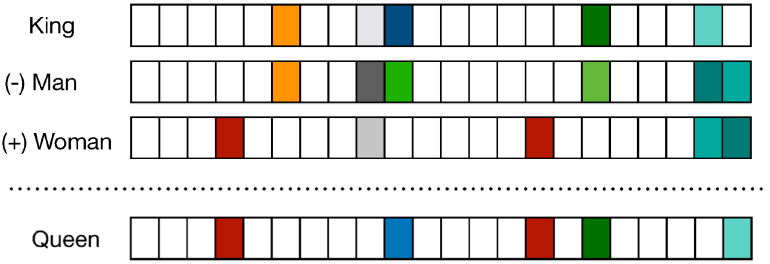
\includegraphics[width=.8\linewidth]{distributed_representation.png}\\
\textbf{Words to Vectors}
\begin{itemize}
    \item Mathematical function maps word to high dimensional Vector
    \item In neural networks, this function is implemented in the Embedding Layer
\end{itemize}
\textbf{Advantage (of vectors)}
\begin{itemize}
    \item Good embedding maps similar/related words to similar regions of the vector space (nearby words have a semantic similarity)
    \item Dot-Product (Skalarprodukt) is a measure of similarity
    \item Possible to add/subtract vectors
\end{itemize}
\textbf{Calculate Similarities between words}
Dot-Product (Skalarprodukt) of 2 Vectors is
\begin{itemize}
    \item maximal when parallel (0\textdegree), both vectors with norm 1 results in max value 1
    \item zero when orthogonal (90\textdegree)
    \item minimal (negative) when opposite directions (180\textdegree) both vectors with norm 1 results in max value -1
\end{itemize}
\textbf{Cosine Distance}
\begin{itemize}
    \item Way to calculate how similar two words (vectors) are
\end{itemize}
cat: A, dog: B \\
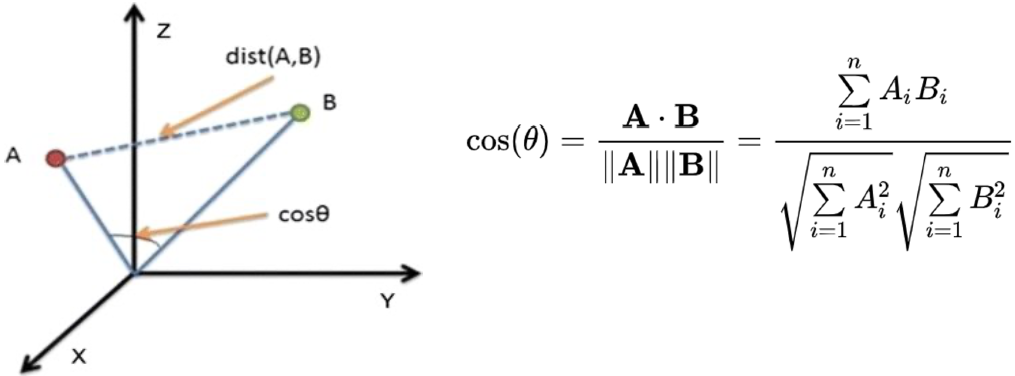
\includegraphics[width=\linewidth]{cosine_distance.png}
Example \\
A: (3, 6, 2, 1), B: (2, 7, 2, 0) \\
$A \cdot B = 6 + 42 + 4 + 0 = 52$ \\
$|| A || || B || = \sqrt{(9 + 36 + 4 + 1)} * \sqrt{(4 + 49 + 4 + 0)} = 53.38539$ \\
$A * B / ( || A || || B ||) = 0.9740$ \\
high value equals high similarity (to be an animal)



        \columnbreak
        \section{Probability}
\subsection{Random Variables}
\begin{itemize}
    \item Values depend on outcomes of a random phenomenon
    \item Random variable $X$ is a variable that takes a numerical value $x$, which depends on a random experiment
    \item \textcolor{blue}{Discrete} $X$ takes any of a finite set of values ${1.5, 2.123, 6.2, 10}$
    \item \textcolor{blue}{Continous} $X$ takes any value of an uncountable range e.g. real numbers from an interval
\end{itemize}
\textbf{Best we can know}
\begin{itemize}
    \item All possible values
    \item Probability of each value
\end{itemize}
E.g. The discrete random variable $X$ is the number observed when rolling a fair dice.\\
$P(X=x)$ / $P(x)$: $1/6$ for each possible value

\textbf{Joint Probability}
\begin{itemize}
    \item Joint Properties of two random variables
    \item Defined by the Joint Probability Mass Function
\end{itemize}
E.g. Dice1 = 5 AND Dice2 = 4\\
$P_{XY}(5,4) = P_X(5) * P_Y(4) = 1/6 * 1/6 = 1/36$\\
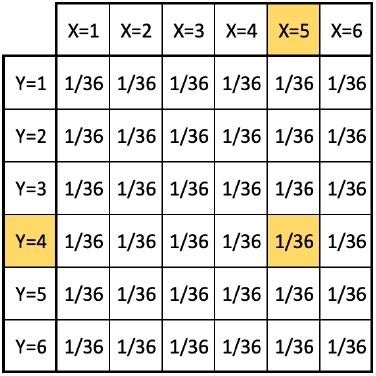
\includegraphics[width=0.5\linewidth]{joint_probability.png} \\
\textbf{Independant random Variables}
\begin{itemize}
    \item Joint Probability is the product of the individual probabilities
\end{itemize}
$P(X,Y) = P(X) * P(Y)$ (only if independant)\\
$P(X,Y,Z) = P(X) * P(Y) * P(Z)$ (only if independant)\\
\textbf{Correlated random Variables}
\begin{itemize}
    \item There are events that are not independant
    \item Such random variables are correlated
    \item $X$: observe clouds (0=no, 1=small, 2=big)
    \item $Y$: observe rain (0=no, 1=light, 2=moderate, 3=heavy)
\end{itemize}
\textbf{Conditional Probability}
\begin{itemize}
    \item One variable is no longer random
    \item X is observed, its value is fixed
    \item Calculate the probabilities of Y given X: $P(Y | X)$
\end{itemize}
$P(X, Y) = P(X | Y) * P(Y)$\\
$P(X, Y) = P(Y | X) * P(X)$\\
$P(Y | X) = \frac{P(X,Y)}{P(X)}$\\
\textbf{Bayes Rule}\\
$P(X|Y)*P(Y) = P(Y|X)*P(X)$\\
Therefore\\
$P(Y|X) = \frac{P(X|Y)*P(Y)}{P(X)}$


\subsection{Probability mass function (PMF)}
Wahrscheinlichkeitsfunktion, a function f(x) that provides the probability for each value x of a discrete random
variable $X$ \\

Graph of a PMF \\
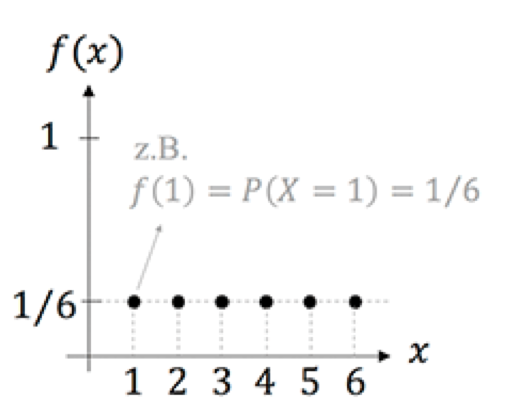
\includegraphics[width=0.2\linewidth]{pmf-graph.png} \\

        \columnbreak
        %\section{Python}

        \section{Data Visualization}
\begin{itemize}
    \item See trends, clusters and local patterns in data
    \item Difficult to see in raw data
    \item Detect outliers and unusual groups
    \item Validate Hypothesis/Conjecture/Theory
\end{itemize}
\vspace{10pt}
\textbf{Important in a Plot}
\begin{itemize}
    \item \textcolor{blue}{X-Axis labels} which data is represented and its units
    \item \textcolor{blue}{Y-Axis labels} which data is represented and its labels
    \item \textcolor{blue}{Title}
    \item \textcolor{blue}{Scale} linear, logarithmic
    \item \textcolor{blue}{Dimensionality of the data 2D / 3D}
\end{itemize}
\vspace{10pt}
\textbf{Dataframe}

a two-dimensional labelled data structure with columns of different types

\subsubsection{Data Analysis Libraries}
\textbf{NumPy}
\begin{itemize}
    \item Package for scientific computing in Python
    \item Multidimensional array object
    \item Routines for fast array operations (sorting, selecting, FFT, linear, ...)
\end{itemize}

\textbf{pandas}
\begin{itemize}
    \item Built on top of NumPy
    \item Routines for accessing tabular data from files (.csv, xls, etc.)
    \item Supports 2-dimensional data (dataframe and series)
    \item Dataframes are something like database tables
\end{itemize}

\textbf{MatPlotLib}
\begin{itemize}
    \item Library for visualizing data
    \item Provides bargraphs, histograms, piecharts, scatter plots, lines, boxplots, heatmaps, ...
\end{itemize}

\textbf{Seaborn}
\begin{itemize}
    \item Extension of MatPlotLib, NumPy and pandas
    \item More user friendly
    \item Plots are aesthetically better
\end{itemize}

\subsubsection{Line Plots}
\begin{itemize}
    \item Bivariate, Continuous
    \item Recognizes trend (pattern of change) (over time)
    \item E.g. Preisgestaltung für Aktienoptionen, Preis von Handys, Bevölkerung eines Lande
\end{itemize}
\subsubsection{Bar Chart}
\begin{itemize}
    \item Used for categorical data
    \item Counting based on each category
    \item E.g. Amount of apps in category Google Play, Apple Store ...
\end{itemize}
\subsubsection{Histogram}
\begin{itemize}
    \item Represents the empirical distribution of a variable
    \item Automatically creates bins (interval) along the range of values
    \item Shows vertical bars to indicate the number of observations per bin
\end{itemize}
\subsubsection{Box Plot (Descriptive Statistics)}

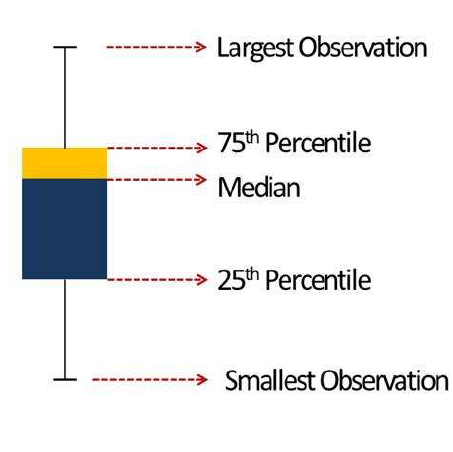
\includegraphics[width=0.5\linewidth]{descriptive_statistics-bx.png}

\textbf{Quartile}

\begin{center}
    $n \cdot p$ ganzzahlig

    $x_p = \frac{1}{2} ( x_{[np]} + x_{[np + 1]})$

    $n \cdot p$ nicht ganzzahlig ($|np|$ auf Ganzzahl abrunden)

    $x_p = x_{[|np|+1]}$ \\
\end{center}

\textcolor{blue}{Quartile 1 (Q1) - 25th Percentile}

$p = 0.25$

25\% der Daten sind kleiner oder gleich diesem Wert. \\

\textcolor{blue}{Quartile 2 (Q2) - 50th Percentile (Median)}

$p = 0.5$

50 \% der Daten sind kleiner oder gleich diesem Wert. Merkmalswert, dessen Merkmalsträger in der Rangordnung aller Merkmalsträger genau die mittlere Position einnimmt. \\

\textcolor{blue}{Quartile 3 (Q3)- 75th Percentile}

$p = 0.75$

75 \% der Daten sind kleiner oder gleich diesem Wert.


\subsubsection{Violin Plots (Descriptive Statistics)}

Wird oftmals verwendet, wenn mehrere Verteilungen von Daten dargestellt werden sollen

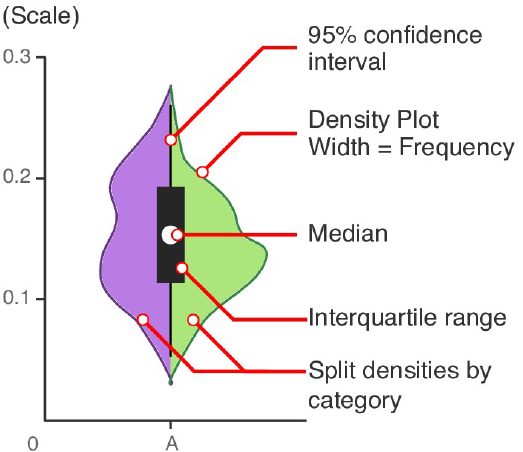
\includegraphics[width=0.5\linewidth]{descriptive_statistics-vio.png}


\subsubsection{Scatter Plot}

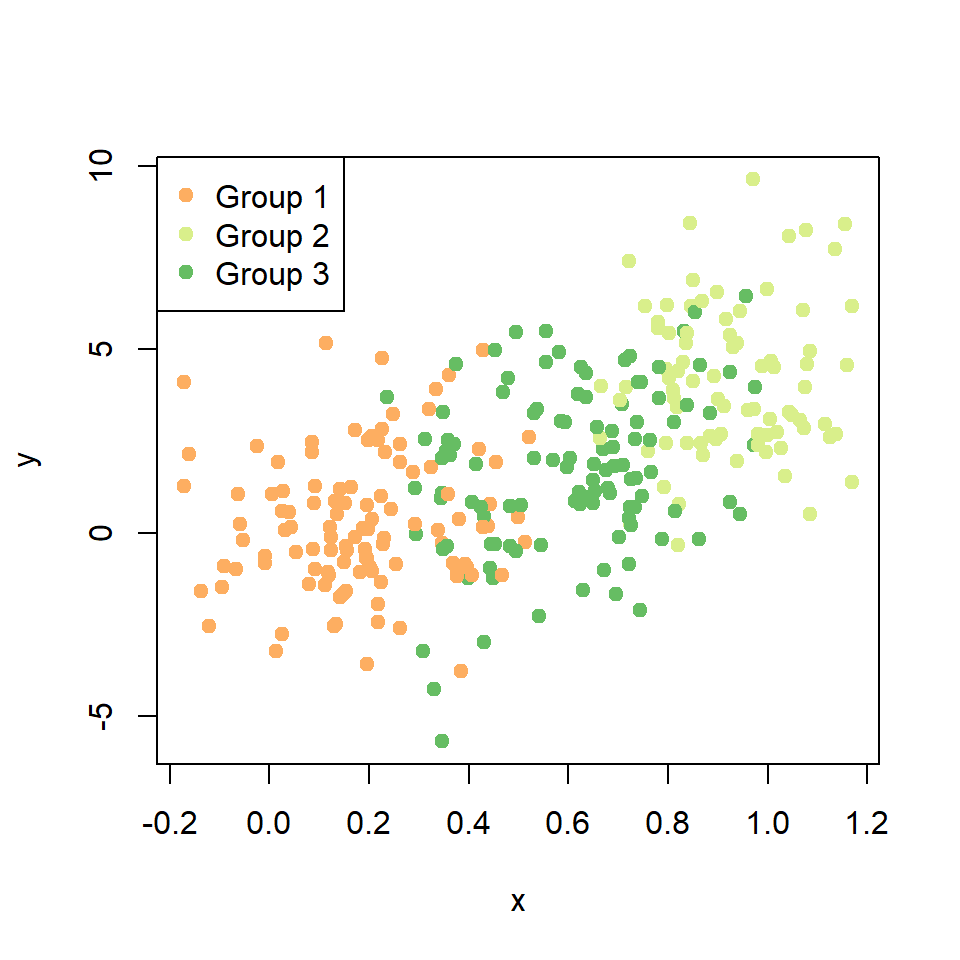
\includegraphics[width=0.7\linewidth]{scatter-plot.png}

\begin{itemize}
    \item Relationship between (two) continuous variables
    \item Helps to get an idea of the degree of correlation between variables
    \item Oftmals nicht hilfreich, wenn Data nichtnumerisch / kategorisch $\rightarrow$ Besser ist in diesem Fall Heat Map
\end{itemize}

        \columnbreak
        \section{Regression}
\subsection{What is a model?}
In ML, we use the term \textbf{model} for any mathematical function that explains the data:\\ 
$y_i = f(x_i)$\\ 
$y_i = f(x_i) + \epsilon_i$\\ 
where $\epsilon_i$ is unexplained noise. It is often assumed that $\epsilon_i$ follows a normal distribution.\\ 
Instead of approximating $y_i$, we calculate an \textbf{estimate} $\hat{y_i}$ (y hat) of the usually unknown $y_i$: \\
\begin{center}
    $\hat{y_i} = f(x)$
\end{center}

\subsubsection{Linear Regression}
\begin{itemize}
    \item Only consideres a linear relationship between input and output
    \item In the simplest case, $x$ and $y$ are scalars and the linear model therefore has only two free parameters
    \item The goal is to identify $a$ (slope) and $b$ (intercept) for which the linear model best explains the data
\end{itemize}
\begin{center}
    $\hat{y_i} = ax_i + b$
\end{center}

\subsubsection{Mean Squared Error (MSE)}
\begin{itemize}
    \item Loss we want to minimize
    \item Usually divided by 2
\end{itemize}
\begin{center}
    $\hat{y_i} = ax_i + b$\\ 
    $e_i = y_i - \hat{y_i}$ \\ 
    The difference $e_i$, called residual\\ 
    $E = \frac{1}{2N} * \displaystyle\sum_{i = 1}^{N} e_i^2$\\
    $E = \frac{1}{2N} * \large\displaystyle\sum_{i = 1}^{N}(\hat{y_i} - (a*x_i + b))^2$
\end{center}

\subsubsection{Correlation and Causality}
\begin{itemize}
    \item Correlation is not causality
    \item Correlation refers to the degree to which a pair of variables are linearly related
    \item Linear regression is a tool to detect correlations between two or more variables
    \item Correlation can be quantified using the Pearson correlation coefficient
\end{itemize}
        \columnbreak
        \section{Optimization}
\begin{itemize}
    \item Training or learning in AI often suggests an algorithm performing some sort of optimization
    \item It is the problem of finding a set of inputs to an objective function that results in a maximum or minimum function evaluation
    \item In our examples the objective is to minimize the loss function
\end{itemize}

\subsection{Gradient Descent}
At any location [a,b] we look at the error-gradient in the neighbourhood of [a,b] and move a (small) step in the direction where the error shrinks the most.
By repeating this procedure, we will eventually arrive at the location where the error is smallest.

\begin{itemize}
    \item Iterative Method/Procedure
    \item Each iteration, the model parameters are updated such as that the Loss (MSE) is reduced
    \item Move along a trajectory which includes fewer points
    \item At each point of the trajectory we evaluate the gradient of the error function
    \item At each iteration, we would have to iterate over all $N = 1'000$ points to calculate the gradient of the loss function.
\end{itemize}

\textbf{Calculate Gradient}

\begin{center}
    $
    \textrm{Gradient of E} = \begin{bmatrix}
                                 \frac{\partial E}{\partial a} \\
                                 \frac{\partial E}{\partial b} \\
    \end{bmatrix}
    $
\end{center}

Calculate these two partial derivatives

\begin{center}
    $\frac{\partial E}{\partial a} = \frac{1}{N}\sum_{i=1}^N (y_i - (a \cdot x_i + b)) \cdot -x_i$
\end{center}

\begin{center}
    $\frac{\partial E}{\partial b} = \frac{1}{N}\sum_{i=1}^N (y_i - (a \cdot x_i + b)) \cdot -1$
\end{center}

\begin{center}
    $
     \textrm{Gradient of E} = \begin{bmatrix}
                                  \frac{\partial E}{\partial a} \\
                                  \frac{\partial E}{\partial b} \\
     \end{bmatrix}
     =\begin{bmatrix}
          \frac{1}{N}\sum_{i=1}^N (y_i - (a \cdot x_i + b))(-x_i) \\
          \frac{1}{N}\sum_{i=1}^N (y_i - (a \cdot x_i + b))(-1) \\
     \end{bmatrix}
    $
\end{center}

\subsection{Stochastic Gradient Descent (SGD)}
we do not need the exact gradient to find a trajectory toward the minimum. Instead, at each iteration we can randomly pick a few datapoints and use them to calculate an approximation of the gradient.
\begin{itemize}
    \item At each iteration, the gradient is calculated on a (randomly selected) subset of the data
    \item For a fixed learning rate, SGD does not converge
\end{itemize}

\textbf{Mini-batches} \\

\begin{itemize}
    \item $1<n<N$
    \item Increasing the batch-size will reduce the variance of the gradient estimation
    \item batch-size $n=1$ yields a very noisy gradient
    \item batch-size $n=N$ is expensive to calculate
    \item often mini-batches of size $n=32$ or $n=64$ are used
\end{itemize}

\textbf{Annealed SGD}
\begin{itemize}
    \item The learning rate alpha is reduced over time
    \item This is called (simulated) annealing
    \item There are different options (called schedules) how to reduce alpha over time
    \item A fixed learning rate $\alpha$ does not converge. The algorithm keeps fluctuating around the minimum. Annealed SGD solves this appearent contradiction by adapting the learning rate. It starts with a large $\alpha$ and reduces it over time
\end{itemize}

\subsubsection{General remarks on SGD}
\begin{itemize}
    \item Gradient-based methods only work if we can express a Loss function as a differentiable function
    \item SGD is dealing with only a single datum at each iteration. This is very inefficient and rarely used.
    \item Batch- or mini-batch gradient-descent is usually used
\end{itemize}

        \columnbreak
        \section{Generalization \& Regularization}
\subsection{Overfitting}
\begin{itemize}
    \item A model that perfectly fits the data does not have to be perfect
    \item In-Sample Error (Trainig error) was minimized (MSE = 0)
    \item Out-of-sample Error (Generalization Error, Test Error) is the MSE of new Data
    \item A good model has a low Generalization Error
    \item Overfitting happens if the MSE of Training Error is small thanks to a complex model but the Generalization Error is large
\end{itemize}
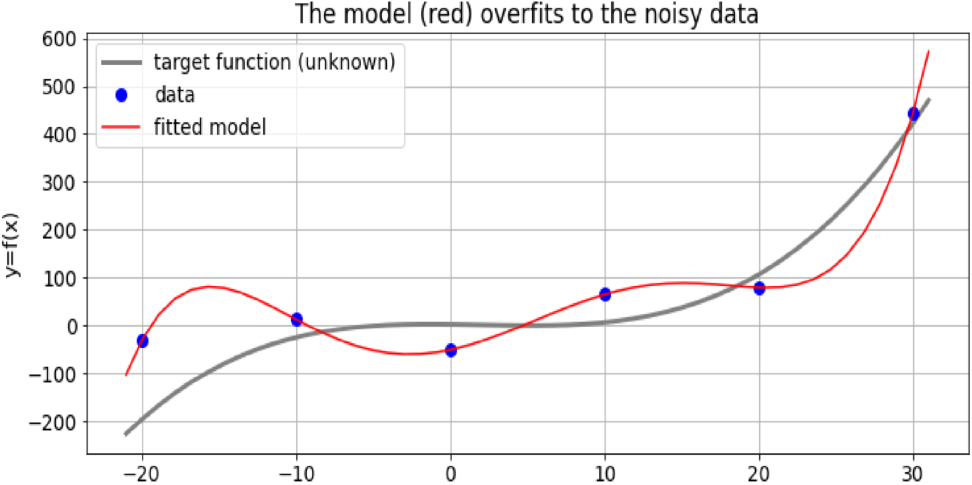
\includegraphics[width=0.9\linewidth]{./img/overfitting.png}

\subsection{Underfitting}
\begin{itemize}
    \item Using a too simple model
    \item In-Sample Error is large
    \item Generalization Error is large
\end{itemize}

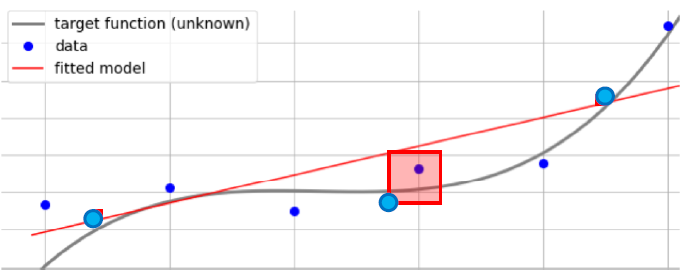
\includegraphics[width=0.9\linewidth]{./img/underfitting.png}

\subsection{Training-Set, Test-Set, Model Evaluation}
\begin{itemize}
    \item The Generalization Error can't be calculated
    \item But Estimated
    \item Split the data into 2 sets
    \begin{itemize}
        \item Training-Set (~80\% of data)
        \item Test-Set (~20\% of data)
    \end{itemize}
\end{itemize}
\textbf{Training:} 
\begin{itemize}
    \item Fit the model to the training set
    \item This minimizes the in-sample error
\end{itemize} 
\textbf{Evaluating}
\begin{itemize}
    \item Using the Test-Set
    \item Produces the Test-Error
    \item This is an estimate of the Generalization Error
\end{itemize}

\subsection{Bias-Variance Trade-off}
\textbf{High Bias}
\begin{itemize}
    \item A too simple model for the given data
\end{itemize}
\textbf{Low Variance}
\begin{itemize}
    \item The model is relatively stable
    \item Very simular model if trained with new data
\end{itemize}
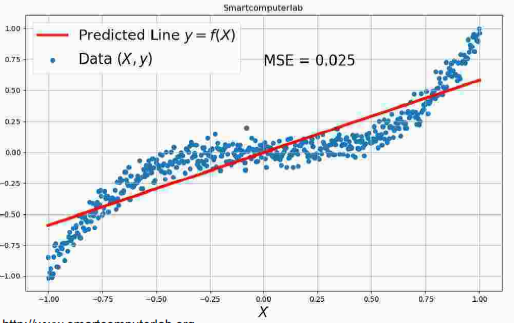
\includegraphics[width=0.6\linewidth]{./img/bias_variance.png}\\
\textbf{Low Bias}
\begin{itemize}
    \item A more complex model can better explain the data
\end{itemize}
\textbf{High Variance}
\begin{itemize}
    \item Given a new datapoint, the MSE can be very large
    \item For a different set with more datapoints, the model may be very different
\end{itemize}
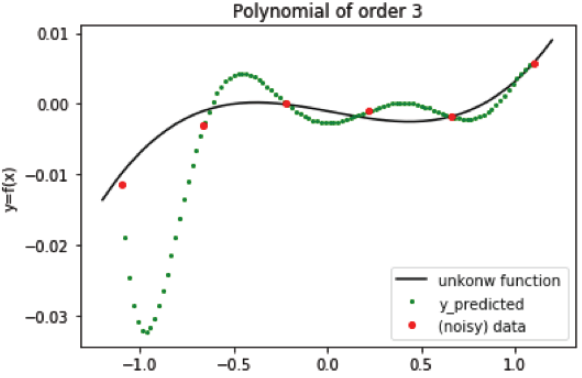
\includegraphics[width=0.6\linewidth]{./img/bias_variance2.png}

\subsubsection{Trade-off}
\begin{itemize}
    \item Higher bias implies lower variance
    \item Lower bias implies higher variance
    \item In practice, all we want is low variance
    \item The model can only be as complex as the data permits
    \item You have to find an optimal balance between bias and variance
\end{itemize}
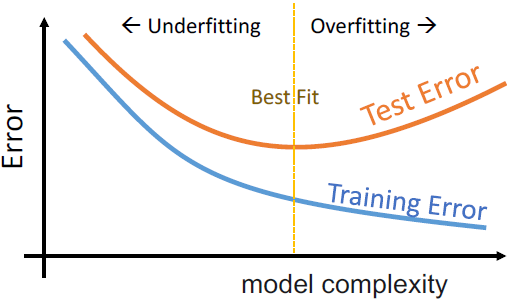
\includegraphics[width=0.6\linewidth]{./img/tradeoff.png}

\subsection{Regularization}
\begin{itemize}
    \item Technique to control the model complexity
    \begin{itemize}
        \item Add a penalty term to the Loss
        \item More complex models get a higher penalty
        \item Add a constrain to the optimization process
        \item \textit{regularized loss} = \textit{MSE + $\lambda$ model-complexity}
    \end{itemize}
\end{itemize}
\begin{center}
    $\displaystyle\sum_{i = 1}^{n} (y_i - \displaystyle\sum_{j = 1}^{p} x_{ij}\beta_j)^2 + \lambda \displaystyle\sum_{j = 1}^{p}\beta_j^2$
\end{center}
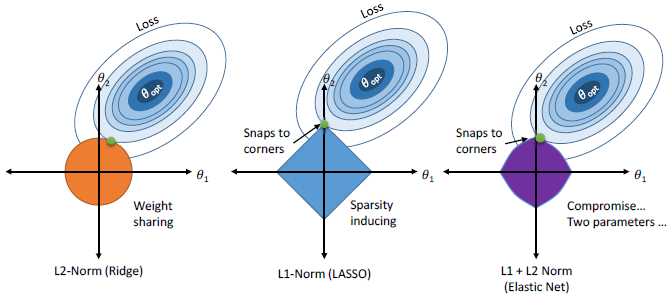
\includegraphics[width=1\linewidth]{./img/regularization.png}

        \columnbreak
        \section{Cross-Validation}
\textbf{Problem with 80/20 Data Separation}
\begin{itemize}
    \item Test Error depends on random set
    \item For different Set, the test error would be different
\end{itemize}
\textbf{With Cross-Validation we can obtain a better estimate of the generalization error}

\columnbreak
\subsection{k-fold Cross-Validation}
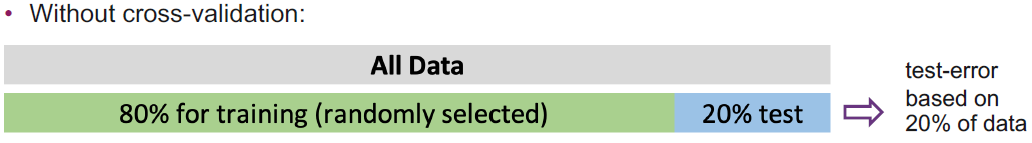
\includegraphics[width=\linewidth]{./img/k_fold.png}
\textbf{With k-Fold Cross-Validation}\\
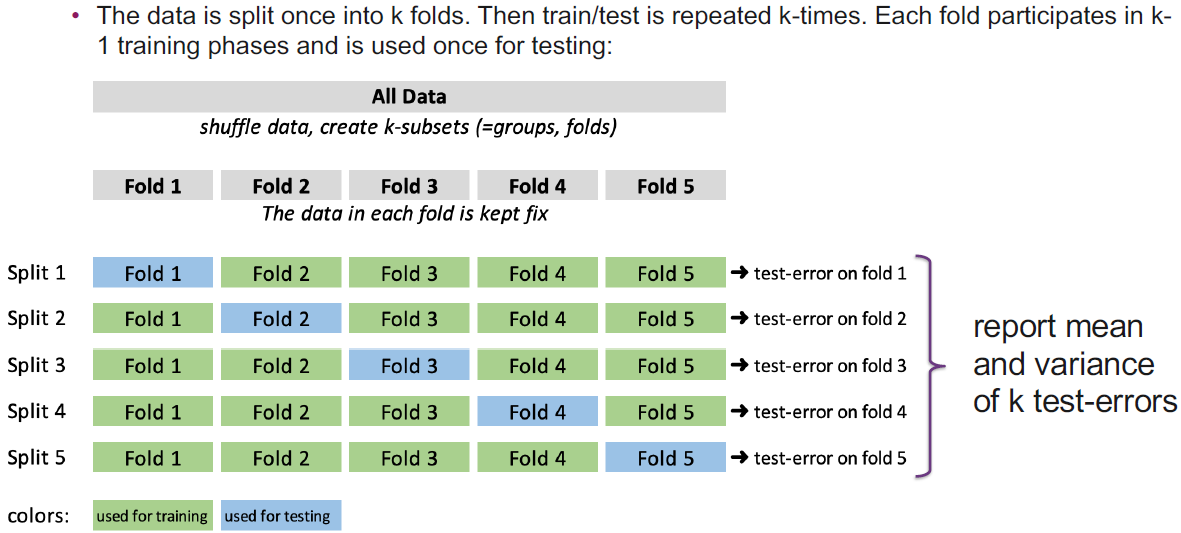
\includegraphics[width=\linewidth]{./img/k_fold2.png}

\subsubsection{Some Comments}
\begin{itemize}
    \item Typical Values for k are 5,10 or N
    \item The data of a fold does not change during procedure
    \item Do not preprocess the whole dataset
    \item Apply the preprocessing pipe-line to each split
\end{itemize}

\section{Artificial Neural Networks (ANN)}
\subsection{Artificial Neurons}
\begin{itemize}
    \item Receives an input vector $[x_1,x_2, ...]$
    \item Each neuron has its own input weights $[w_1, w_2, ...]$ and \textbf{bias} b
    \item Calculates the sum of the weighted input (dot product $\vec{x} * \vec{w}$), adds a bias b, and passes it through a nonlinear activiation function
\end{itemize}
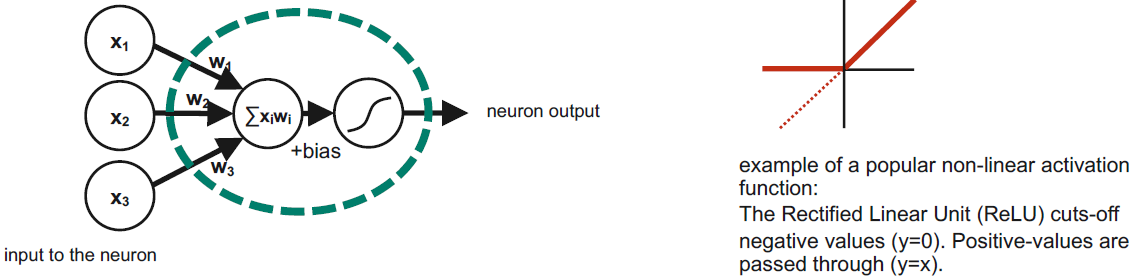
\includegraphics[width=\linewidth]{./img/artificial_neurons.png}

\subsection{Simple ANN}
\includegraphics[width=\linewidth]{./img/ann.png}

\subsection{Traning an ANN}
\textbf{Supervised learning}
\begin{itemize}
    \item For each input $\vec{x}$ we are given the output $\vec{y}$
    \item ANN is initialized with random weights
    \item An optimizer reduces a cost-function (e.g. MSE)
    \item At every iteration, and for every single weight $w$ and bias $b$, the partial derivative needs to be calculated. (Backpropagation)
\end{itemize}
\includegraphics[width=\linewidth]{./img/train_ann.png}

        \columnbreak
        
\section{Artificial Neural Networks (ANN)}
An ANN is a data-structure to define arbitrarily complex mathematical functions

\subsection{Artificial Neurons}
\begin{itemize}
    \item Receives an \textcolor{blue}{input vector $[x_1,x_2, ...]$}
    \item Each neuron has its own \textcolor{blue}{input weights $[w_1, w_2, ...]$} and \textcolor{blue}{bias b} (=intercept)
    \item Neuron calculates the sum of the weighted input (dot product $\vec{x} \cdot \vec{w}$), adds a bias b, and passes it through a \textcolor{blue}{nonlinear activation function}
\end{itemize}
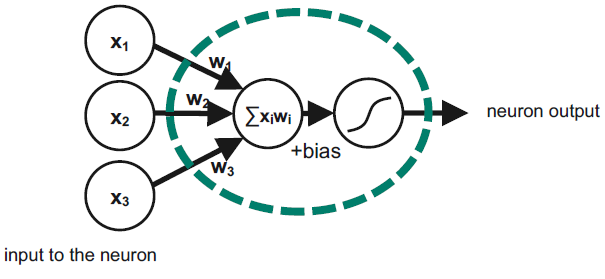
\includegraphics[width=0.6\linewidth]{artificial_neurons-1.png} \\

\textbf{Activation Function (ReLU)}

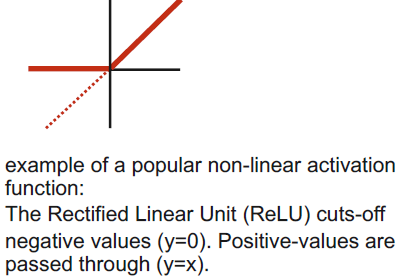
\includegraphics[width=0.6\linewidth]{artificial_neurons-2.png}


\subsection{Simple Artificial Neural Network (ANN)}
\includegraphics[width=\linewidth]{ann.png}

\textcolor{blue}{Trainable parameters} input vectors and input weights

\subsection{Training an ANN}
\textbf{Supervised learning}
\begin{itemize}
    \item Data with label
    \item For each input $\vec{x}$ we are given the output $\vec{y}$
    \item ANN is initialized with random weights
    \item An optimizer (e.g. SGD) reduces a cost-function (e.g. MSE)
    \item \textcolor{blue}{At every iteration, and for every single weight $w$ and bias $b$, the partial derivative needs to be calculated.} (Backpropagation algorithm)
\end{itemize}
\includegraphics[width=\linewidth]{train_ann.png}

        \columnbreak
        \section{Logistic Regression}
Classification method

\subsection{Binary Classification}
Decision with 2 possible outcomes (yes, no)

\begin{itemize}
    \item Hail in Lausanne (yes/no)
    \item Master admission (admission / no admission)
    \item Based on different data / entity
\end{itemize}
$y = 1$ implies yes/accepted/admission, $y = 0$ implies no/rejected \\
$P(y = 1, x_1 = 4.5, x_2 = 5, x_3 = 5.5)$\\

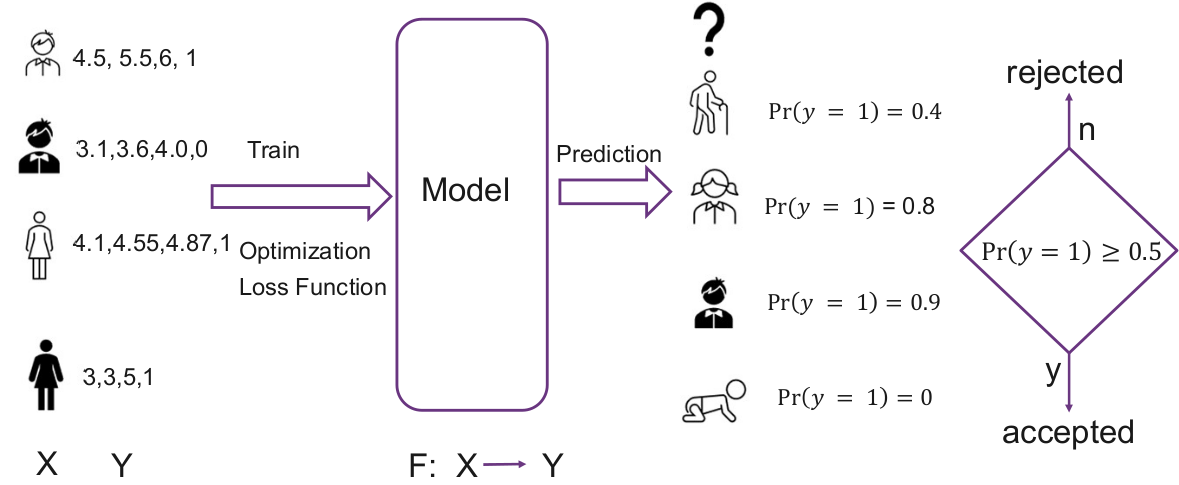
\includegraphics[width=\linewidth]{binary-classification.png}

\subsection{Predicting Probabilities: Logistic Regression}

\textbf{Decision using Linear Regression}
\begin{itemize}
    \item Train the model with gradient descent
    \item \textcolor{red}{Bad Idea!}
    \item Models the response (y) and post process the response (e.g.\ by thresholding) to compute the probability
    \item MSE minimiert den Unterschied von $\hat{y}$ und $y$, was nichts mit der Classification Wahrscheinlichkeit zu tun hat
\end{itemize}
\vspace{10pt}
\textbf{Sigmoid function (the model)}

\begin{itemize}
    \item Values between 0 and 1. $y$ is interpreted as probability
    \item \textcolor{blue}{Function is not parametrized}
    \item Has a single input value
\end{itemize}

\begin{center}
    $sigmoid(y) = \frac{1}{1 + e^{-y}}$
\end{center}
$y$ is

\begin{itemize}
    \item calculated from the input data
    \item a linear combination of the input features, with one feature $ax_i + b$ with D dimensions $y_i=\sum_{d=0}^{d=D}w_d \cdot x_i^d$
    \item e.g. $y = w_1 x_1 + w_2 x_2 + w_3 x_3 + w_4 x_4$
\end{itemize}
\vspace{10pt}
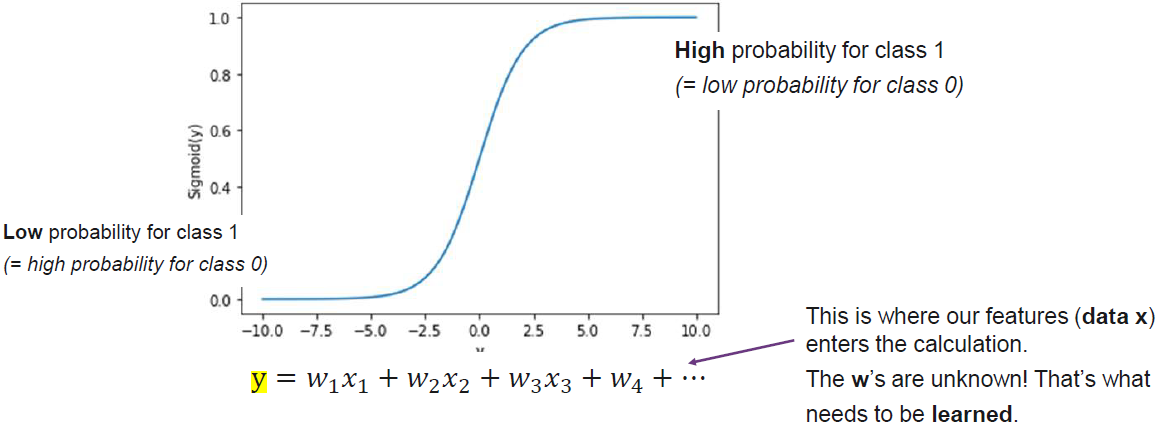
\includegraphics[width=\linewidth]{sigmoid.png} \\

\textbf{Probabilities}
\begin{itemize}
    \item We can write the estimated probability
    \item For a prediction we can write
\end{itemize}
\begin{center}
    $P(x) = \frac{1}{1 + e^{-(W^{T}x)}}$
\end{center}
\vspace{10pt}
\begin{center}
    For example $Pr(y_i = 1 | x_i; w) = \Large \frac {1}{1 + e^{-(w_0 + w_1 \cdot x_{i, 1} + w_2 \cdot x_{i, 2} + w_3 \cdot x_{i, 3})}}$
\end{center}

\subsection{Optimization: Maximum Likelihood Estimation - Loss Function}
\begin{itemize}
    \item \textcolor{blue}{Given all the data points (X,Y) we want to maximize the probability that all the predictions are correct.}
    \item For each of the training data, we want to maximize the likelihood of correct prediction
    \item We can use \textcolor{blue}{Gradient Descent to find optimal $W$}
\end{itemize}
\vspace{10pt}
\begin{center}
    Minimize $cost(W) = E = -\frac{1}{N}\sum_{i=1}^N (y_i \cdot log(p_i)) + (1 - y_i) \cdot log(1 - p_i))$
\end{center}
\vspace{10pt}
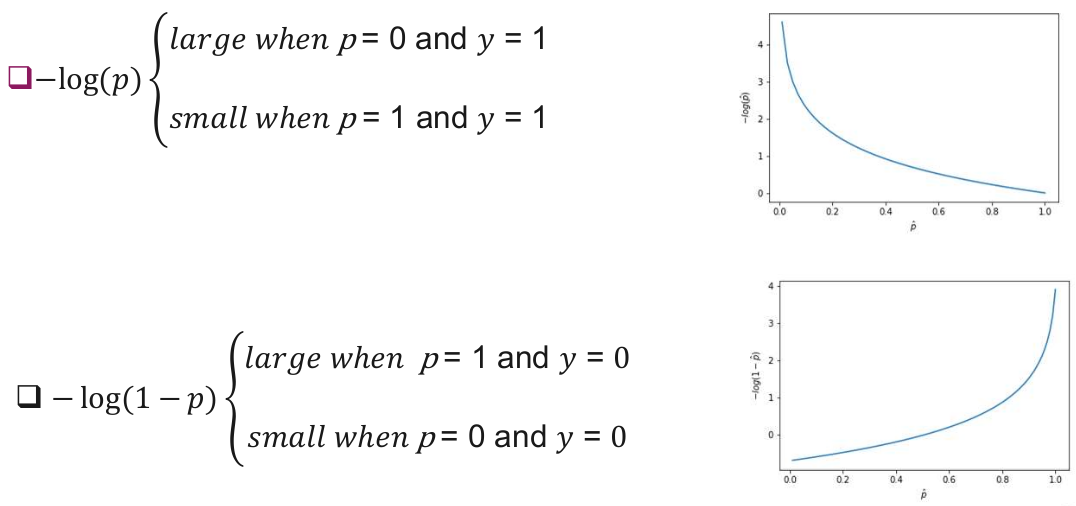
\includegraphics[width=\linewidth]{likelihood-cost.png}

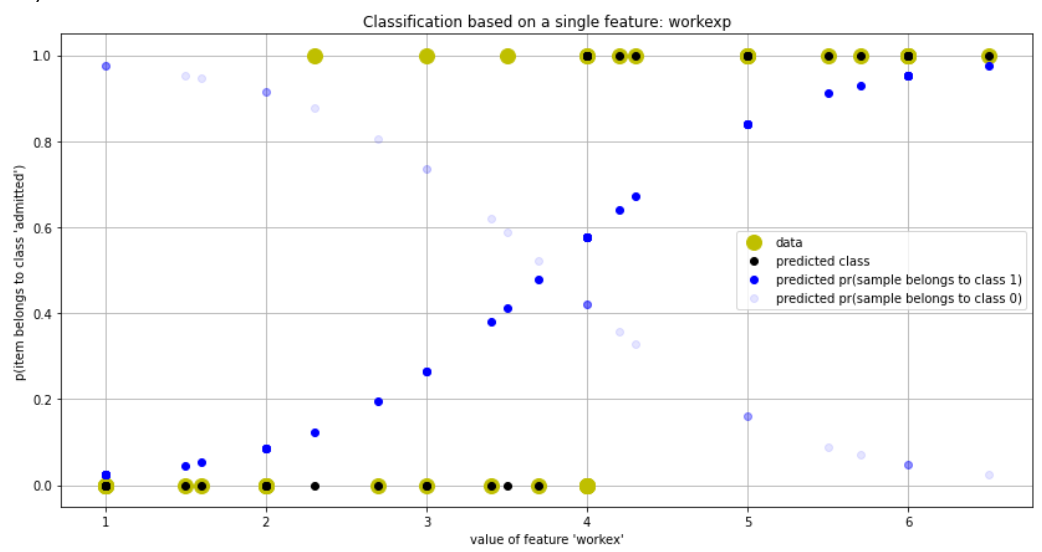
\includegraphics[width=\linewidth]{classification-based-diagram.png}

        \columnbreak
        \section{Classifier Evaluation}
\subsection{Confusion Matrix}
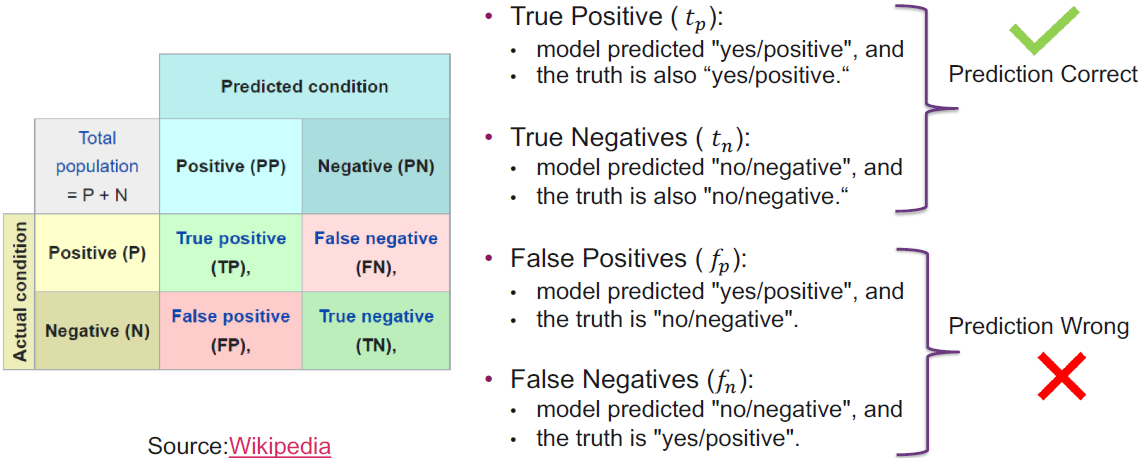
\includegraphics[width=\linewidth]{./img/confusion_matrix.png}
\textbf{Mean Accuracy:}
\begin{itemize}
    \item How often is the classifier correct?
    \item $A = (t_p + t_n) / n$
\end{itemize}
\textbf{Mean Error:}
\begin{itemize}
    \item How often is the classifier wrong?
    \item $E = (f_p + f_n) / n$
\end{itemize}
\textbf{Precision:}
\begin{itemize}
    \item When the prediction is 1, how often is it correct?
    \item $P = t_p / (t_p + f_p)$
\end{itemize}
\textbf{Sensitivity, Recall, True Positive Rate (TPR):}
\begin{itemize}
    \item How often the prediction is 1 when it's actually 1
    \item $R = t_p / (t_p + f_n)$
\end{itemize}
\textbf{Miss Rate, False Negative Rate (FNR)}
\begin{itemize}
    \item $MR = 1 - TPR$
\end{itemize}

\subsection{Why Accuracy is not enough?}
\begin{itemize}
    \item If the prediction is constant the accuracy may still look decent
    \item E.g. allways predict false
    \item 90\% of the data is false
    \item Accuracy = 90\% (decent)
    \item Precision = 0
    \item Recall = 0
\end{itemize}

\subsection{Precision vs. Recall}
\begin{itemize}
    \item Increasing precision reduces Recall and vice versa
    \item Threshold is a business decision (depending on goals)
\end{itemize}

\subsection{Receiver Operating Characteristics}
\begin{itemize}
    \item Defined by FPR and TPR as x and y axes
    \item Visualizes tradeoff between TP (benefits) and FP (cost)
\end{itemize}
\begin{center}
    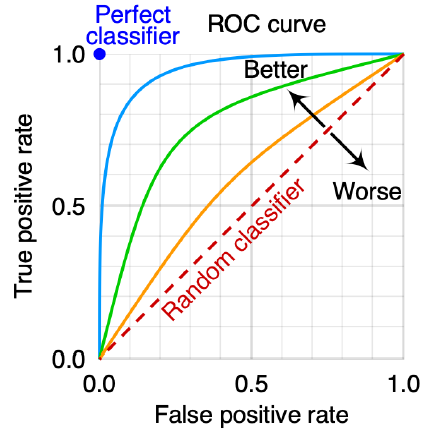
\includegraphics[width=0.4\linewidth]{./img/roc.png}
\end{center}
\textbf{Area under the curve}
\begin{itemize}
    \item Area under the ROC curve
    \item Shows how well the TPR and FPR is looking in the aggregate
    \item The greater the area under the curve, the higher the quality of the model
    \item The greater the area, the higher the ratio of TP to FP
\end{itemize}

\section{KNN}
\subsection{Linear Seperability}
\includegraphics[width=1\linewidth]{./img/linear_sep.png}

\begin{itemize}
    \item Based on logistic regression model, you can draw a line
    \item This is the Linear decision boundary
    \item If a simple line perfectly seperates the classes, then the classes are said to be linearely seperable
\end{itemize}

\subsection{Non-Linear decision boundary}
\begin{itemize}
    \item When classes are not linearly seperable
    \item Resort to polynomial terms
\end{itemize}

\subsection{k-Neares Neighbors (KNN)}
\begin{itemize}
    \item A datapoint is know by the company it keeps
    \item Computes $k$ nearest neighbours
    \item Returns the most frequent class of the $k$ neighbours
\end{itemize}
\includegraphics[width=0.8\linewidth]{./img/knn.png}
\subsubsection{Distance Metric}
\begin{itemize}
    \item Cosine Distance
    \item Manhattan Distance
    \item Euclidean Distance (most used)
    \item Minkowski Distance
\end{itemize}
\subsubsection{Advantages}
\begin{itemize}
    \item Easy and simple ML model
    \item Few hyperparameters to tune
\end{itemize}

\subsubsection{Disadvantages}
\begin{itemize}
    \item $k$ should be wisely selected
    \item Large computation cost during runtime if sample size is large
    \item Not efficient for high dimensional datasets
    \item Proper scaling should be provided for fair treatment among features
\end{itemize}

\subsubsection{Hyperparameters}
\begin{itemize}
    \item \textbf{K Value}: how many neighbours to participate in the KNN algo.
    \item \textbf{Distance Function}: Euclidean distance is most used
\end{itemize}
        \columnbreak
        \section{K-Nearest Neighbour (KNN)}
Classification method

\subsection{Linear Separability}
\includegraphics[width=1\linewidth]{linear_sep.png}

\begin{itemize}
    \item Based on logistic regression model, you can draw a line
    \item This is the Linear decision boundary
    \item If a simple line perfectly seperates the classes, then the classes are said to be linear separable
\end{itemize}

\subsection{Non-Linear decision boundary}
\begin{itemize}
    \item When classes are not linearly separable
    \item Resort to polynomial terms
\end{itemize}

\subsection{k-Neares Neighbors (KNN)}
\begin{itemize}
    \item A datapoint is know by the company it keeps
    \item Computes $k$ nearest neighbours
    \item Returns the most frequent class of the $k$ neighbours
\end{itemize}
\includegraphics[width=0.8\linewidth]{knn.png}
\textbf{Process}
\begin{enumerate}
    \item Load the training and test data
    \item Choose value of $k$ (number of nearest neighbours to consider for classification)
    \item For each test data points $x_{test}$
        \subitem For all training data $x_{train}$ calculate $d(x_{test}, x_{train})$ with distance metric
        \subitem Sort training data in ascending order of distance
        \subitem Choose first $k$ data points from sorted training data
        \subitem Choose most frequently occurring class from $k$ data points as classification result
\end{enumerate}

\textbf{Distance Metric}
\begin{itemize}
    \item Cosine Distance $cost \theta = \frac{x_1 \cdot x_2}{||x_1|| ||x_2||}$
    \item Manhattan Distance $d_M = \sum_{i=1}^{n}| x_{1,n} - x{2,n} |$
    \item Euclidean Distance (most used) $d_E = \sqrt{\sum_{i=1n}^{}(x_{1,n} - x_{2,n})^2}$
    \item Minkowski Distance
\end{itemize}
\textbf{Advantages}
\begin{itemize}
    \item Easy and simple ML model
    \item Few hyperparameters to tune
\end{itemize}

\textbf{Disadvantages}
\begin{itemize}
    \item $k$ should be wisely selected
    \item Large computation cost during runtime if sample size is large
    \item Not efficient for high dimensional datasets
    \item Proper scaling should be provided for fair treatment among features
\end{itemize}

\textbf{Hyperparameters}
\begin{itemize}
    \item \textcolor{blue}{K Value} how many neighbours to participate in the KNN algo.
    \item \textcolor{blue}{Distance Function} Euclidean distance is most used
\end{itemize}

        \columnbreak
        \section{Clustering}
\subsection{Unsupervised Learning}
\begin{itemize}
    \item We are given Data (features, x) wihout labels (y)
    \item It learns something through the structure of the data
    \item \textbf{The goal} of unsupervised learning is to self-discover patterns from the data
\end{itemize}

\textbf{Clusters}
\begin{itemize}
    \item Data points which have shared properties
    \item Fall into one cluster or one alike group
    \item Similar Data Points are close together
    \item Group $n$ data points into $k_c$ number of clusters
\end{itemize}
\textbf{Applications}
\begin{itemize}
    \item Social Network Analysis
    \item Astronomical Data
    \item Marked segmentation
    \item Recommendation systems
\end{itemize}
\subsection{Naive K-means}
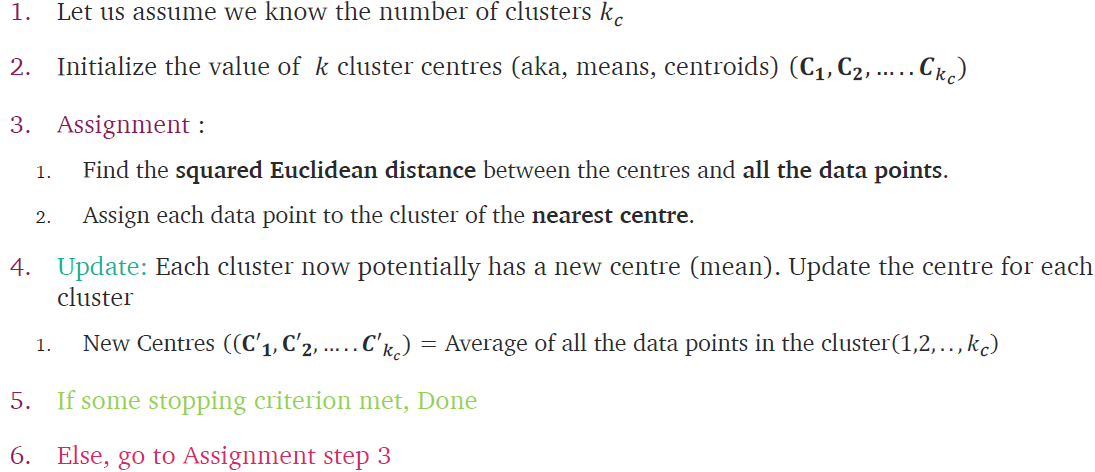
\includegraphics[width=\linewidth]{k-means.png}

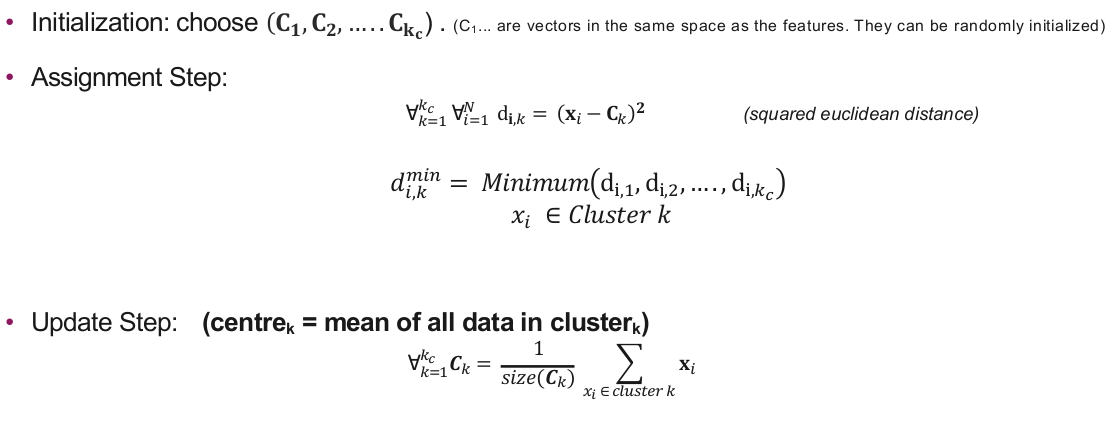
\includegraphics[width=\linewidth]{clusters-formal-maths.png}

\textbf{Stopping Criterion}
\begin{itemize}
    \item When centres don't change (time consuming)
    \item The datapoints assigned to specific cluster remains the same (takes too much time)
    \item The distance of datapoints from their centres $>=$ treshold we have set
    \item Fixed number of iterations have reached (choose wisely)
\end{itemize}

\textbf{Initialization}
\begin{itemize}
    \item Performance depends on the random initialization
    \item Some seeds can result in a poor convergence rate
    \item Some seeds can converge to suboptimal clustering
    \item If centres are very close, it takes a lot of iterations to converge
    \item Initialize randomly, run multiple times
\end{itemize}

\textbf{Standardization of data}
\begin{itemize}
    \item Features with large values may dominate the distance value
    \item Features over small values will have no impact
    \item Normalize values!
\end{itemize}

\subsection{Sklean k-means}
\textbf{Initialization}
\begin{itemize}
    \item Init = K-means++
    \item Only initialization of the centroids will change
    \item Chosen centroids should be far from each other
\end{itemize}
\textbf{max\_iter}
\begin{itemize}
    \item Number of iterations before stopping
\end{itemize}
\textbf{n\_init}
\begin{itemize}
    \item Number of time the k-means algorithm will be run with different centroid seeds
\end{itemize}

\subsection{Evaluate Cluster Quality}
\begin{itemize}
    \item Make clusters so that for each cluster the distance of each cluster member from its center is minimizes
\end{itemize}
\textbf{Inertia or within-cluster sum-of-squares (WCSS)}
\begin{itemize}
    \item Sum of squared distances of samples (each point) to their closest center
    \item As small as possible
\end{itemize}

\begin{minipage}[t]{0.5\linewidth}
    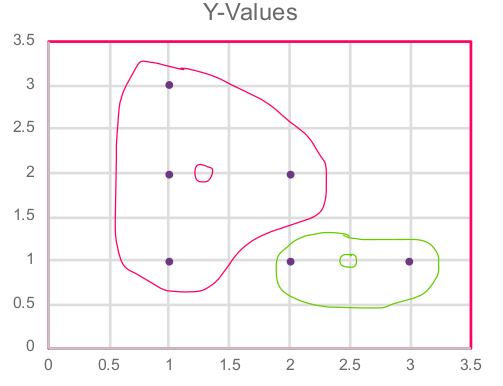
\includegraphics[width=\linewidth]{wcss-diagram.png}
\end{minipage}
\begin{minipage}[t]{0.5\linewidth}
    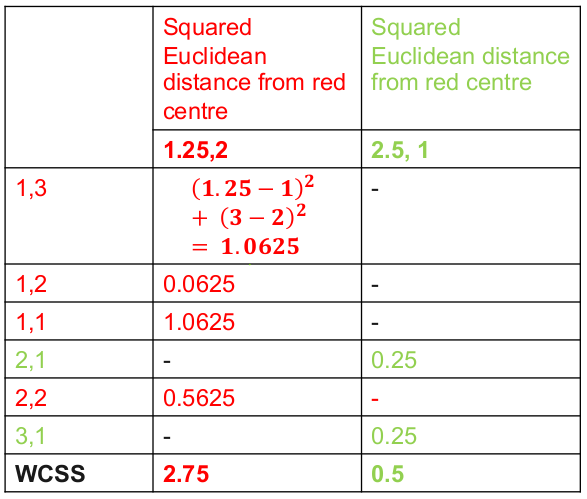
\includegraphics[width=\linewidth]{wcss-table.png}
\end{minipage}


\textbf{Silhouette Score}
\begin{itemize}
    \item How far the datapoints in one cluster are from the datapoints in another cluster
    \item Silhouette Score of a point: $\frac{b-a}{max(a,b)}$
    \item a: average intra-cluster distance (distance between each point within)
    \item b: average inter-cluster distance (distance between a cluster and its nearest neighbour)
\end{itemize}
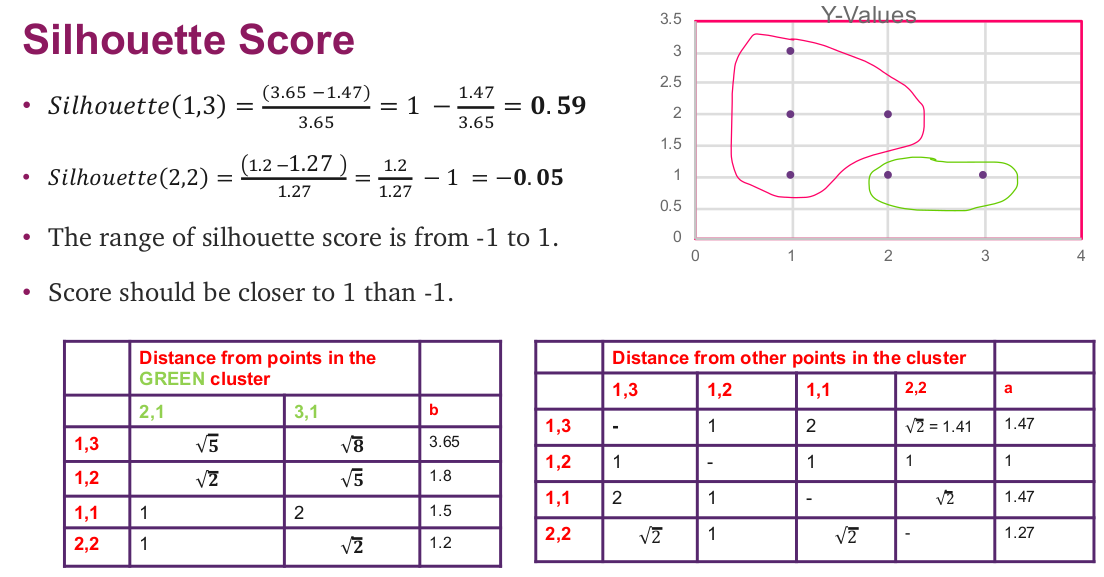
\includegraphics[width=\linewidth]{silhouette-score.png}

        \columnbreak
        \section{Ensemble Methods}
\begin{itemize}
    \item Suppose we have many different weak models (better than random)
    \item Get prediction from all of them and take a vote
    \item Class with most votes is the predicted class
    \item Commonly used towards the end of a project
    \item \textcolor{blue}{Requirement} enough models / diverse models
\end{itemize}
\vspace{10pt}
\textbf{Wisdom of Crowd}
\begin{itemize}
    \item Suppose you have a difficult question
    \item Ask many people and aggregate the answer
    \item This might work very well instead of finding the best suited person
\end{itemize}
\vspace{10pt}
\textbf{Transfer}
\begin{itemize}
    \item Wisdom of Crowd can be applied to ML
    \item Instead of finding the best model, aggregate the results of weak models
    \item Aggregate predictions of regressors or classifiers
    \item Might get better accuracy than the best predictor
    \item Ensemble: group of predictors
\end{itemize}
\vspace{10pt}
\textbf{Aggregate predictions}
\begin{itemize}
    \item \textcolor{blue}{Hard voting} Predict class with most votes
    \item \textcolor{blue}{Soft voting} Predict class with the highest class probability
\end{itemize}

\subsection{Sampling}
\textbf{Bagging (Bootstrap Aggregating)}
\begin{itemize}
    \item Sampling with replacement (a data point can be selected more than once)
    \item Allows data points to be used several times
\end{itemize}
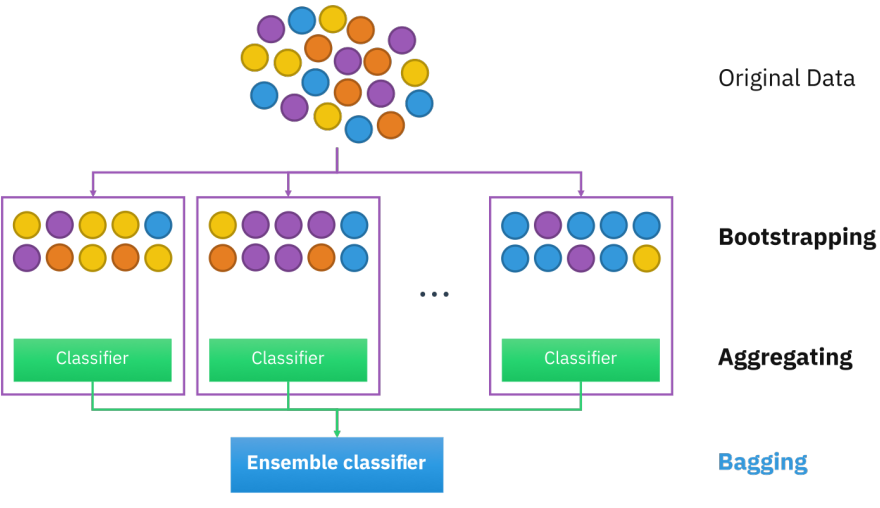
\includegraphics[width=0.8\linewidth]{bagging.png} \\

\textbf{Pasting}
\begin{itemize}
    \item Sampling without replacement (a data point can be selected only once)
\end{itemize}
\vspace{10pt}
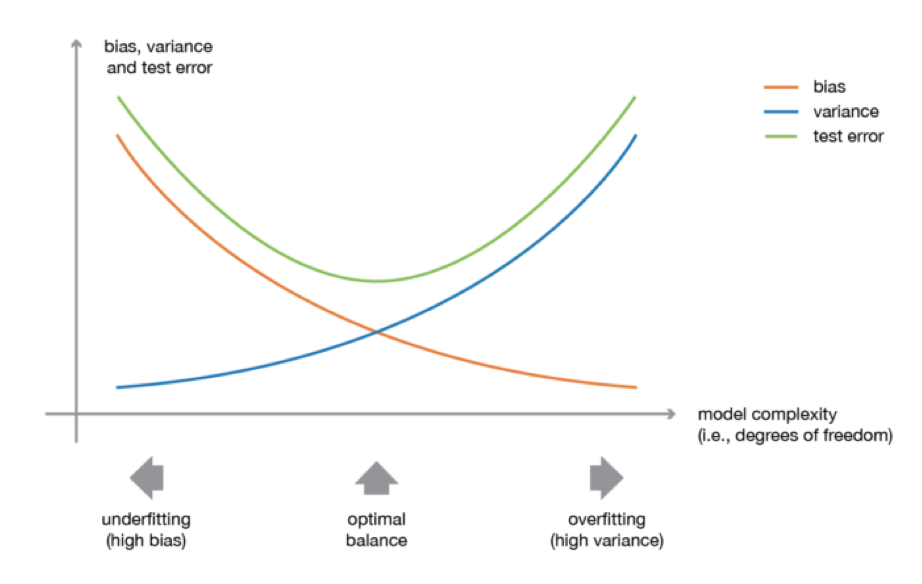
\includegraphics[width=\linewidth]{ensamble-bagging.png}

\begin{enumerate}
    \item Die individuellen Modelle haben relative hohe Bias und tiefe Variance
    \item Bootstrap (wiederverwendung von Daten) verringert die Variance
    \item Die Aggregation erhöht potenziell die Aussagekraft des Modells und verringert daher die Bias
\end{enumerate}

\subsection{No free lunch theorem}
\textit{No single machine learning algorithm is universally the best-performing algorithm for all problems}

\begin{itemize}
    \item No single algorithm will solve all your machine learning problems better than every other algorithm.
    \item All models are only as good as the assumptions that they were created with and the data that was used to train them.
    \item Simpler models like \textcolor{blue}{logistic regression} have more bias and tend to \textcolor{blue}{underfit}, while more complex models like \textcolor{blue}{neural networks} have more variance and tend to \textcolor{blue}{overfit}.
    \item The best models for a given problem are somewhere in the middle of the two bias-variance extremes.
    \item To find a good model for a problem, you may have to try different models and compare them using a robust cross-validation strategy.
\end{itemize}
\vspace{10pt}
\textbf{Out of Bag (oob) Evaluation}
\begin{itemize}
    \item Using Bagging
    \item Some Data Points may not be used at all
    \item Use them for evaluation
\end{itemize}


    \end{multicols*}
\end{document}

























